\subsection{Sviluppo}
	\subsubsection{Descrizione}
	Il processo di sviluppo contiene le attività ed i compiti che devono essere svolti per produrre il software richiesto. Esso viene svolto in conformità allo standard ISO/IEC 12207:1995, comprendendo perciò le seguenti attività:
	\begin{itemize}
		\item{Analisi;}
		\item{Progettazione;}
		\item{Codifica.}
	\end{itemize}

	In particolare, l'obiettivo del team è sviluppare un prodotto\ped{\textit{G}} software che superi i test, soddisfi le richieste ed i requisiti, fissati dal Proponente\ped{\textit{G}}.

    \subsubsection{Attività}
    	\subsubsubsection{Analisi}
	L'attività di analisi consiste nello studio dei bisogni e delle fonti del dominio applicativo. Ha come obiettivo una modellazione concettuale del sistema mediante l'assegnazione di requisiti a parti distinte del sistema.

        \subsubsubsection*{Analisi dei Requisiti}
          	Nell'\AdR{} gli Analisti individuano ed elencano tutti i requisiti richiesti dal Proponente\ped{\textit{G}} per il progetto in questione. Tali requisiti possono derivare da:
     \begin{itemize}
           		\item{capitolato\ped{\textit{G}} d'appalto;}
				\item{verbali di riunioni interne o esterne;}
				\item{casi d'uso\ped{\textit{G}}.}
    	\end{itemize}

          	E sono fondamentali per:
        \begin{itemize}
       		\item{descrivere lo scopo del lavoro;}
			\item{fornire ai Progettisti riferimenti specifici ed affidabili;}
			\item{fissare funzionalità concordate con il cliente;}
			\item{fornire una base per raffinamenti successivi al fine di garantire un miglioramento continuo;}
			\item{facilitare le revisioni del codice;}
			\item{stimare i costi in base alla quantità di lavoro prevista.}
       	\end{itemize}

        \subsubsubsection*{Casi d'uso}
		Dopo aver identificato i casi d'uso\ped{\textit{G}}, è compito degli Analisti elencare questi ultimi con un grado di precisione che va dal generale al particolare, usando la struttura:
		\begin{itemize}
	    	\item{\textbf{codice identificativo}};
	    	\item{\textbf{titolo}};
	    	\item{\textbf{diagramma UML\ped{\textit{G}}}};
	    	\item{\textbf{attori primari}};
	    	\item{\textbf{attori secondari}};
	    	\item{\textbf{descrizione}};
	    	\item{\textbf{scenario principale}};
    		\item{\textbf{specializzazioni (se presenti)}};
	    	\item{\textbf{inclusioni (se presenti)}};
	    	\item{\textbf{estensioni (se presenti)}};
	    	\item{\textbf{precondizione}};
	    	\item{\textbf{postcondizione}}.
		\end{itemize}

		\noindent Ogni caso d'uso\ped{\textit{G}} dev'essere corredato da un codice identificativo, che segue la dicitura:
		\begin{center}
			\textbf{UC[codice\_padre].[codice\_figlio]}
		\end{center}

		\noindent Dove:
		\begin{itemize}
         	\item{\textbf{Codice padre}: numero che identifica univocamente i casi d'uso\ped{\textit{G}} generici;}
         	\item{\textbf{Codice figlio}: numero progressivo che identifica i sottocasi. Può a sua volta includere altri livelli.}
		\end{itemize}

        \subsubsubsection*{Requisiti}
		Ogni requisito emerso durante l'attività di analisi dev'essere descritto dalla seguente struttura:
           	\begin{itemize}
                  	\item{codice identificativo;}
                  	\item{fonti;}
                  	\item{relazioni di dipendenza con altri requisiti;}
                  	\item{descrizione;}
                  	\item{importanza.}
    			\end{itemize}

           	\noindent Ogni requisito dev'essere corredato da un codice identificativo, che segue la dicitura:
			\begin{center}
				\textbf{R[Importanza][Tipologia][Codice]}
			\end{center}

			Dove:
			\begin{itemize}
			   	\item{\textbf{Importanza}: indica il grado di importanza del requisito ai fini del progetto. Può assumere i valori:}
			   	\begin{itemize}
			           	\item{\textbf{1}: requisito obbligatorio ai fini del progetto, irrinunciabile per gli stakeholders;}
			           	\item{\textbf{2}: requisito desiderabile: non strettamente necessario ai fini del progetto ma che porta valore aggiunto;}
			           	\item{\textbf{3}: requisito opzionale, contrattabile più avanti nel progetto.}
			   	\end{itemize}

			   	\item{\textbf{Tipologia}: classe a cui appartiene il requisito in questione. Può assumere i valori:}
			   	\begin{itemize}
			   		\item{\textbf{F}: funzionale;}
			   		\item{\textbf{P}: prestazionale;}
			   		\item{\textbf{Q}: qualitativo;}
			   		\item{\textbf{V}: vincolo.}
			   	\end{itemize}

			   	\item{\textbf{Codice}: identificatore univoco del requisito}.
			\end{itemize}
         \noindent Il codice stabilito secondo la convenzione precedente, una volta associato ad un requisito, non può più essere modificato. \\

            \noindent Inoltre per ogni requisito bisogna indicare:
            \begin{itemize}
               	\item{\textbf{descrizione}}: breve descrizione del requisito, strutturata in maniera da evitare ambiguità;

               	\item{\textbf{classificazione}}: indica il grado di importanza del requisito considerato. Sebbene tale informazione sia già presente nell'identificativo, la sua ripetizione rende la lettura più semplice e scorrevole;

               	\item{\textbf{fonti}}:
               	\begin{itemize}
               		\item \textit{capitolato}\ped{\textit{G}}: requisito indicato nel capitolato\ped{\textit{G}};
               		\item \textit{interno}: requisito individuato dagli analisti;
               		\item \textit{caso d'uso}\ped{\textit{G}}: il requisito è stato estrapolato da uno o più casi d'uso\ped{\textit{G}}. In questo caso vengono riportati gli identificativi dei casi d'uso\ped{\textit{G}} considerati;
               		\item \textit{verbale}\ped{\textit{G}}: si tratta di un requisito individuato a seguito di un incontro tra i membri del gruppo o di una richiesta di chiarimento con il Proponente\ped{\textit{G}}.
               		In questo caso è riportato il codice identificativo presente nella tabella delle decisioni dei verbali considerati.
               	\end{itemize}
            \end{itemize}

        \subsubsection*{Diagrammi UML}
        I diagrammi UML\ped{\textit{G}} devono essere realizzati utilizzando la versione del linguaggio \textit{v2.0}.
        Per garantire leggibilità è richiesto che gli Analisti si occupino di creare i diagrammi UML\ped{\textit{G}}
        rispettando le seguenti indicazioni:
        \begin{itemize}
           	\item distribuire in modo omogeneo gli elementi all'interno dello spazio disponibile, mantenendo un margine minimo;
           	\item dove possibile, allineare i vari elementi sia in senso verticale sia in orizzontale;
           	\item impostare i collegamenti in uscita da ogni elemento ad angolo retto.
        \end{itemize}


    \subsubsubsection{Progettazione}
        L'attività di progettazione definisce una soluzione del problema presentato soddisfacente per tutti gli stakeholders, in relazione ai requisiti specificati nel documento \AdR{} \textit{2.0.0}. Questo garantisce che il prodotto\ped{\textit{G}} sviluppato soddisfi le proprietà e i bisogni specificati dal Proponente\ped{\textit{G}}.
        La progettazione ha quindi come obiettivo l'elaborazione di una struttura adeguata per il sistema, e si divide in:
        \begin{itemize}
        	\item{\textbf{Progettazione Architetturale}}: vengono svolte operazioni di incremento, verifica dei requisiti e progettazione ad alto livello di un'architettura adeguata alla realizzazione del progetto. La Technology Baseline\ped{\textit{G}} del progetto si ottiene alla fine di questo periodo;
        	\item{\textbf{Progettazione di Dettaglio}}: vengono svolte operazioni di incremento, verifica dei documenti redatti; vengono definite le specifiche di dettaglio dell'architettura del prodotto\ped{\textit{G}}, partendo dalla Tecnology Baseline\ped{\textit{G}}. Particolare attenzione viene data alla codifica di tale prodotto\ped{\textit{G}} ed alla creazione di un manuale utente. La Product Baseline\ped{\textit{G}} del progetto si ottiene alla fine di questo periodo;
        \end{itemize}
    	I rispettivi output sono:
        \begin{itemize}
           	\item{\textbf{\TB{}}\ped{\textit{G}}: contiene le specifiche della progettazione ad alto livello e la Proof of Concept;}
			\item{\textbf{\PB{}}\ped{\textit{G}}: approfondisce l'attività di progettazione precedentemente trattata nella Technology Baseline\ped{\textit{G}}, specifica le definizioni delle classi e definisce i test necessari alla verifica.}
   		\end{itemize}

  \subsubsubsection*{Technology Baseline}
  Deve contenere:
  \begin{itemize}
		\item \textbf{Tracciamento delle componenti}: viene rappresentata la relazione tra ogni requisito ed il componente che lo soddisfa, dimostrando concretamente il loro soddisfacimento;
		\item \textbf{Test di integrazione}: vengono definite delle classi di verifica per accertarsi che ogni componente del sistema funzioni come previsto;
		\item \textbf{Tecnologie utilizzate}: devono essere descritte le tecnologie utilizzate, specificandone l'utilizzo nel progetto e le motivazioni per cui sono state scelte.
		\item \textbf{Poc (Proof of Concept)}: eseguibile funzionale alla dimostrazione dell'adeguatezza delle scelte architetturali;
  \end{itemize}

  \subsubsubsection*{Product Baseline}
  Deve contenere:
  \begin{itemize}
		\item{\textbf{Diagrammi UML}\ped{\textit{G}}}: usati per rendere più chiare le scelte progettuali adottate e ridurre le ambiguità. Possono essere:
				\begin{itemize}
							\item{diagrammi di attività}: descrivono la logica procedurale di un flusso di operazioni, aiutando a descrivere gli aspetti dinamici dei casi d'uso\ped{\textit{G}};
				\item{diagrammi delle classi:} descrivono le classi presenti all'interno del sistema, soffermandosi sui loro metodi, attributi e relazioni;
				\item{diagrammi dei package}: descrivono le relazioni di dipendenza presenti tra classi raggruppate in package diversi, ossia in raggruppamenti di un numero arbitrario di elementi in unità di livelllo più alto;
			\item{diagrammi di sequenza}: descrivono la collaborazione di un gruppo di oggetti che devono implementare collettivamente un comportamento;
		\end{itemize}
		\item \textbf{Design pattern}\ped{\textit{G}}: vengono esplicitati chiaramente i design pattern\ped{\textit{G}} utilizzati per l'architettura, accompagnandoli con una descrizione ed un diagramma così da esporne il significato e la struttura;
		\item \textbf{Definizione delle classi}: ogni classe viene descritta illustrandone lo scopo e le funzionalità;
		\item \textbf{Tracciamento delle classi}: ogni requisito viene tracciato, in modo da garantire che ogni classe ne soddisfi almeno uno;
		\item \textbf{Test di unità}: vengono definiti dei test di unità per verificare che le componenti del sistema funzionino come previsto.
  \end{itemize}

    	\subsubsection*{Diagrammi delle classi}
    	I diagrammi delle classi devono descrivere le tipologie di oggetti presenti all'interno del sistema e le relazioni di dipendenza tra essi presenti.
    	Ogni classe viene rappresentata tramite un rettangolo tripartito in senso orizzontale,
    	che conterrà rispettivamente:
    	\begin{enumerate}
    		\item{\textbf{nome della classe}}: che deve essere univoco, scritto con la lettera maiuscola e in inglese. Nel caso in cui la classe sia astratta, il nome deve essere scritto in italico; nel caso in cui si tratti invece di un'interfaccia, il nome dovrà essere preceduto dal termine \texttt{<<interface>>};

    		\item{\textbf{attributi (opzionali)}}: rappresentano lo stato interno della classe. Ogni attributo deve essere indicato nel seguente modo:
    		\begin{center}
    			\textbf{visibilità nome : tipo [molteplicità] = default \{proprietà aggiuntive\}}
    		\end{center}
    		dove:
    			\begin{itemize}
    				\item{\textbf{visibilità}}: visibilità dell'attributo rispetto all'esterno della classe, può essere pubblica, protetta o privata;
    				\item{\textbf{nome}}: nome dell'attributo;
  					\item{\textbf{tipo}}: tipo dell'attributo;
				\item{\textbf{molteplicità (opzionale)}}: numero di occorrenze dell'attributo all'interno della classe;
				\item{\textbf{default(opzionale)}}: eventuale valore predefinito dell'attributo;
				\item{\textbf{proprietà aggiuntive}}: eventuali informazioni aggiuntive relative all'attributo considerato;
    			\end{itemize}

    		\item{\textbf{operazioni (opzionali)}}: rappresentano le azioni che la classe è in grado di compiere. Ogni operazione deve essere indicata nel seguente modo:
    			\begin{center}
    				\textbf{visibilità nome (lista-parametri) : tipo-ritorno \{proprietà aggiuntive\}}
    			\end{center}
    		dove:
    			\begin{itemize}
    				\item{\textbf{visibilità}}: visibilità dell'operazione rispetto all'esterno della classe, può essere pubblica, protetta o privata;
    				\item{\textbf{nome}}: nome dell'operazione;
    				\item{\textbf{lista-parametri}}: lista di parametri dell'operazione; per ogni parametro dovranno essere indicate le seguenti proprietà:
     				\begin{itemize}
     					\item{\textbf{direzione (opzionale)}}: modalità di accesso al parametro, può essere in lettura, in scrittura o entrambe; di default è in lettura;
     					\item{\textbf{nome}}: nome del parametro;
     					\item{\textbf{tipo}}: tipo del parametro;
     					\item{\textbf{default (opzionale)}}: eventuale valore di default del parametro;
     				\end{itemize}
    				\item{\textbf{tipo-ritorno}}: tipo di ritorno della funzione considerata;
				\item{\textbf{proprietà aggiuntive(opzionali)}}: eventuali informazioni aggiuntive relative alla funzione;
    			\end{itemize}
    	\end{enumerate}
    	Le varie classi possono essere collegate tra di loro tramite apposite frecce, che esplicitano le relazioni di dipendenza presenti tra esse. In particolare, i gradi di dipendenza considerati sono:
    	\begin{itemize}
    		\item{\textbf{dipendenza}}: indicata con la freccia tratteggiata, si ha quando la classe utilizza un oggetto della classe con cui si relaziona;
    		\item{\textbf{aggregazione}}: indicata con la freccia "a diamante" vuota, si ha quando la classe considerata presenta come attributo almeno un riferimento alla classe con cui si relaziona;
    		\item{\textbf{composizione}}: indicata con la freccia "a diamante" piena, si ha quando la classe contiene come attributo almeno un oggetto della classe con cui si relaziona;
    		\item{\textbf{associazione}}: indicata con una linea semplice, si ha quando la classe crea e utilizza un oggetto della classe con cui si relaziona;
    		\item{\textbf{generalizzazione}}: indicata con la freccia vuota, viene usata per indicare relazioni di tipo "Is-A".
    	\end{itemize}

    	\subsubsection*{Diagrammi dei package}
    	Ogni package deve essere rappresentato tramite un rettangolo con un'etichetta per il nome, in inglese e scritta in minuscolo. Ogni package può contenere al suo interno altri package o classi. \\
    	Le dipendenze tra package devono essere indicate con frecce tratteggiate che dovrebbero seguire tutte le medesima direzione, in modo da evitare la creazione di dipendenze cicliche.

    	\subsubsection*{Diagrammi di attività}
    	I diagrammi di attività permettono di descrivere i processi che compongono l'applicazione software attraverso dei grafi in cui i nodi rappresentano le azioni e gli archi l'ordine in cui esse sono eseguite.
    	Gli elementi usati in tali diagrammi sono i seguenti:
    	\begin{itemize}
    		\item{\textbf{nodo iniziale}}: rappresentato da un pallino pieno, porta alla generazione di un token ed è il punto d'inizio dell'esecuzione dell'attività;
    		\item{\textbf{activity}}: rappresenta un'azione all'interno dell'attività, viene indicata  da un rettangolo che ne contiene la descrizione;
    		\item{\textbf{subactivity}}: è rappresentata da un rettangolo che ne contiene il nome, viene usata per riferirsi ad una sottoattività il cui diagramma deve essere fornito separatamente;
    		\item{\textbf{branch}}: tali nodi modellano delle decisioni, vengono indicati tramite dei rombi vuoti e generalmente distinguono due branch. Il test che deve essere soddisfatto normalmente viene indicato da un'etichetta posta di fianco al nodo di branch;
    		\item{\textbf{merge}}: punto in cui i rami generati da un branch si uniscono, vengono rappresentati nello stesso modo dei nodi di branch;
    		\item{\textbf{fork}}: punto in cui l'attività si parallelizza senza vincoli di esecuzione temporale, viene indicato da una lunga linea orizzontale o verticale. Consuma un token e ne genera uno per ogni percorso in uscita;
    		\item{\textbf{join}}: rappresentato allo stesso modo del fork, è un punto in cui avviene la sincronizzazione di processi paralleli. Consuma un token per ogni percorso in entrata e genera un solo token;
    		\item{\textbf{pin}}: rappresentato da un quadratino da cui entrano o escono frecce, indica la produzione o consumo di un parametro, il cui tipo va indicato di fianco;
    		\item{\textbf{segnali}}: vengono rappresentati tramite due figure "a incastro", la prima (non bloccante) per l'emissione del segnale, la seconda (bloccante) per la ricezione dello stesso. Rappresenta un evento esterno;
    		\item{\textbf{timeout}}: sono rappresentati da una clessidra, permettono di modellare timeout ed eventi ripetuti;
    		\item{\textbf{nodo di fine flusso}}: rappresentato da un cerchio vuoto con una X al centro. Porta al consumo di un token e rappresenta un punto di terminazione di un percorso di esecuzione; non causa la terminazione dell'esecuzione dell'attività;
    		\item{\textbf{nodo finale}}: viene rappresentato da due cerchi concentrici: il più esterno vuoto e il più interno pieno. Porta al consumo di un token e rappresenta il punto di terminazione dell'esecuzione dell'attività.
    	\end{itemize}

    	\subsubsection*{Diagrammi di sequenza}
    	I diagrammi di sequenza permettono di descrivere la collaborazione di un gruppo di oggetti che devono implementare collettivamente un comportamento. \\
    	Tali diagrammi devono essere letti verticalmente, dall'alto al basso, in modo da simulare lo scorrere del tempo. Ognuno degli oggetti coinvolti viene indicato tramite un rettangolo, che contiene il nome a lui associato. \\
    	All'interno del diagramma è consigliato l'utilizzo delle barre di attivazione, in modo da rendere immediatamente visibile a chi osserva lo stato di attività del diagramma. 	\\
    	La collaborazione tra gli oggetti rappresentati è resa possibile tramite lo scambio di messaggi, che viene indicato da apposite frecce. Un messaggio può essere di una delle seguenti tipologie:
    	\begin{itemize}
    		\item{\textbf{messaggio sincrono}}: viene indicato tramite una freccia piena, corrisponde alla chiamata sincrona di un metodo. Il chiamante deve attendere la risposta del chiamato prima di continuare l'esecuzione;
    		\item{\textbf{messaggio asincrono}}: viene indicato tramite una freccia, corrisponde ad una chiamata asincrona. Il chiamante non deve aspettare la risposta del chiamato per continuare l'esecuzione;
    		\item{\textbf{messaggio di ritorno}}: indicato con una freccia tratteggiata, rappresenta il ritorno di un metodo chiamato;
    		\item{\textbf{messaggio di creazione}}: indicato con una freccia tratteggiata sormonata da \texttt{<<create>>}, rappresenta la creazione di un nuovo oggetto;
    		\item{\textbf{messaggio di distruzione}}: freccia piena sormontata da \texttt{<<destroy>>}, indica la distruzione di un oggetto.
    	\end{itemize}

    	\noindent Per modellare in maniera più dettagliata le interazioni tra gli oggetti si consiglia l'utilizzo dei frame d'interazione. Ognuno di tali frame è caratterizzato dalle seguenti proprietà:
    	\begin{itemize}
    		\item{\textbf{guardia}}: indica la condizione di attivazione del frame;
    		\item{\textbf{etichetta}}: viene usata per indicare la tipologia del frame d'interazione considerato. Le tipologie possibili sono:
    		\begin{itemize}
    			\item{\textbf{alt}}: rappresenta un'alternativa tra più frame; viene eseguito solo quello per cui si verifica la condizione;
    			\item{\textbf{opt}}: rappresenta l'esecuzione opzionale di un frame, che avviene solo se la condizione specificata si verifica;
    			\item{\textbf{par}}: indica frammenti da eseguire in parallelo;
    			\item{\textbf{loop}}: indica che il frammento può essere eseguito più volte, la base dell'iterazione è indicata dalla guardia;
    			\item{\textbf{region}}: rappresenta una regione critica, il frammento può essere eseguito da un solo thread alla volta;
    			\item{\textbf{neg}}: indica un'iterazione non valida;
    			\item{\textbf{ref}}: si riferisce ad un'interazione definita in un altro diagramma;
    			\item{\textbf{sd}}: utilizzato per racchiudere un intero diagramma di sequenza.
    		\end{itemize}
    	\end{itemize}

    	\subsubsubsection*{Qualità dell'architettura}
    	In seguito alla definizione dei requisiti, che consolida le funzionalità richieste, ci si occupa della realizzazione dell'architettura del sistema. Tale architettura dovrà godere delle seguenti proprietà:
    	\begin{itemize}
    		\item{\textbf{sufficienza}}: deve soddisfare i requisiti definiti nel documento \AdR{} \textit{2.0.0};
    		\item{\textbf{comprensibilità}}: deve essere capibile da tutti gli stakeholder;
    		\item{\textbf{modularità}}: deve essere suddivisa in parti chiare e ben distinte;
    		\item{\textbf{robustezza}}: deve essere in grado di sopportare ingressi diversi, sia da parte dell'utente che dell'ambiente;
    		\item{\textbf{flessibilità}}: deve permettere di essere modificata senza sostanziali modifiche e a costi contenuti al variare dei requisiti;
    		\item{\textbf{efficienza}}: deve gestire le risorse in maniera da ridurre eventuali sprechi;
    		\item{\textbf{affidabilità}}: l'architettura deve garantire una buona usabilità del prodotto\ped{\textit{G}} una volta implementata;
    		\item{\textbf{disponibilità}}: la manutenzione delle sue parti deve richiedere un tempo limitato e non andare ad affliggere il corretto funzionamento di tutto il sistema;
    		\item{\textbf{sicurezza}}: non deve presentare gravi malfunzionamenti o essere vulnerabile ad intrusioni;
    		\item{\textbf{semplicità}}: ogni sua parte deve contenere solo il necessario e nulla di superfluo;
    		\item{\textbf{incapsulazione}}: costituita da componenti le cui informazioni interne non sono visibii da fuori;
    		\item{\textbf{coesione}}: composta in maniera che le parti con obiettivo comune siano raggruppate insieme;
    		\item{\textbf{basso accoppiamento}}: composta da parti distinte che devono essere indipendenti tra di loro, in modo che l'architettura possa subire modifiche a costi contenuti;
    	\end{itemize}

   	\subsubsubsection{Codifica}
    Questa attività ha come scopo normare l'effettiva realizzazione del prodotto\ped{\textit{G}} software richiesto. Tramite questa attività si concretizza la soluzione architetturale elaborata durante la progettazione, mediante la programmazione vera e propria.
    Gli sviluppatori, durante l' implementazione, dovranno attenersi alle norme di programmazione stabilite in maniera tale da:
    \begin{itemize}
       	\item ottenere codice leggibile ed uniforme per i programmatori;
       	\item agevolare le fasi di manutenzione, verifica e validazione;
       	\item fornire un prodotto\ped{\textit{G}} conforme ai requisiti indicati dal Proponente\ped{\textit{G}};
       	\item migliorare la qualità del prodotto\ped{\textit{G}}.
   	\end{itemize}

   	\noindent La scrittura del codice dovrà inoltre perseguire gli obiettivi di qualità stabiliti nel documento \textit{\PdQ{} 2.0.0}, in modo da garantire una buona qualità del codice.
    	\subsubsection*{Stile di codifica}
   \begin{itemize}
         \item{\textbf{indentazione}: i blocchi innestati devono essere correttamente indentati, usando per ciascun livello di indentazione quattro (4) spazi, fatta eccezione per i commenti. Ogni programmatore dovrà configurare adeguatamente il proprio IDE\ped{\textit{G}} al fine di rispettare tale norma;}
		\item{\textbf{parentesizzazione}: le parentesi di delimitazione dei costrutti vanno inserite in linea e non al di sotto di essi;}
		\item{\textbf{lunghezza dei metodi}: ove possibile, preferire metodi brevi (poche righe di codice) e che assolvano il minor numero di compiti possibile;}
		\item{\textbf{univocità dei nomi}: classi, variabili e metodi devono avere un nome univoco ed esplicativo (nome parlante), al fine di evitare ambiguità e consentire ad eventuali lettori di comprendere lo scopo di quel preciso elemento, anche senza conoscenze informatiche pregresse;}
		\item{\textbf{classi}: le parole componenti i nomi delle classi devono iniziare con la lettera maiuscola (e.g. NomeClasse);}
		\item{\textbf{costanti}: le costanti devono essere scritte usando solo lettere maiuscole (e.g. COSTANTE). Nel caso siano composte da più parole, queste devono essere separate dal carattere speciale underscore (e.g. NOME\_COSTANTE);}
		\item{\textbf{metodi}: i nomi dei metodi devono iniziare con una lettera minuscola e, nel caso 	siano composti da più parole, quelle successive devono iniziare con una lettera maiuscola (e.g. nomeMetodo);}
		\item{\textbf{lingua}: le parti testuali di codice ed i commenti ad esso riferiti devono essere scritti in lingua inglese;}
        \item{\textbf{ricorsione}: l'uso della ricorsione va evitato quanto più possibile.}
	\end{itemize}

	\noindent I componenti \textit{Etherless-cli} ed \textit{Etherless-server} dovranno essere codificati in TypeScript\ped{\textit{G}}, seguendo la Airbnb\ped{\textit{G}} JavaScript\ped{\textit{G}} Style Guide e lo strumento di analisi statica del codice ESLint\ped{\textit{G}}. \\
	Per quanto riguarda \textit{Etherless-smart}, questo dovrà essere sviluppato in Solidity\ped{\textit{G}}, seguendo la relativa style guide presente nel sito ufficiale.

\subsubsection{Metriche}
	\subsubsubsection{Metriche di analisi dei requisiti}
	\subsubsection*{Percentuale dei Requisiti Obbligatori Soddisfatti}
		\begin{itemize}
			\item{\textbf{Descrizione}}: la metrica indica la percentuale di requisiti obbligatori soddisfatti sui requisiti totali;
			\item{\textbf{unità di misura}}: la metrica viene espressa in percentuale;
			\item{\textbf{formula}}: $ PROS = \displaystyle\frac{\#requisiti\_obbligatori\_soddisfatti}{\#requisti\_obbligatori\_totali}\times100$;
			\item{\textbf{risultato}}: il risultato è compreso tra 0\% e 100\%, in particolare:
				\begin{itemize}
					\item una valore inferiore al 100\%, indica la presenza di alcuni requisiti obbligatori non ancora soddisfatti;
					\item una valore pari al 100\%, indica che tutti i requisiti obbligatori presentati sono stati soddisfatti.
				\end{itemize}
		\end{itemize}

	\subsubsubsection{Metriche di progettazione}
		\subsubsection*{Coupling Between Objects (CBO)}
		\begin{itemize}
			\item{\textbf{Descrizione}}: la metrica CBO indica il numero di classi accoppiate ad una data classe;
			\item{\textbf{unità di misura}}: la metrica viene espressa tramite un numero intero;
			\item{\textbf{risultato}}: in linea generale si può dire che:
			\begin{itemize}
				\item un valore pari a 0 indica che la classe non ha alcuna relazione con nessun'altra classe presente all'interno del sistema;
				\item un valore compreso tra 1 e 4 indica che la classe presenta un basso livello di accoppiamento;
				\item un numero maggiore di 4 indica che la classe presenta un livello medio/alto di accoppiamento, che potrebbe complicarne il test e la manutenzione.
			\end{itemize}
		\end{itemize}

		\subsubsection*{Structural Fan-In (SFIN)}
		\begin{itemize}
			\item{\textbf{Descrizione}}: la metrica SFIN indica il numero di componenti che utilizzano un dato modulo\ped{\textit{G}};
			\item{\textbf{unità di misura}}: la metrica viene espressa tramite un numero intero;
			\item{\textbf{risultato}}: un valore elevato di SFIN è indice di un riutilizzo consistente della componente considerata;
		\end{itemize}

		\subsubsection*{Structural Fan-Out (SFOUT)}
		\begin{itemize}
			\item{\textbf{Descrizione}}: la metrica SFOUT indica il numero di componenti utilizzate dal modulo\ped{\textit{G}} considerato;
			\item{\textbf{unità di misura}}: la metrica viene espressa tramite un numero intero;
			\item{\textbf{risultato}}: un valore elevato di SFOUT è indice di un eccessivo livello di accoppiamento della componente;
		\end{itemize}

	\subsubsubsection{Metriche di codifica}
	\subsubsection*{Complessità ciclomatica}
	\begin{itemize}
		\item{\textbf{Descrizione}}: la metrica è indice della complessità di una porzione di codice;  in particolare rappresenta il numero di cammini linearmente indipendenti attraverso il grafo di controllo di flusso;
		\item{\textbf{unità di misura}}: la metrica viene espressa tramite un numero intero;
		\item{\textbf{formula}}: $ v(G) = e - n + 2p $, dove:
			\begin{itemize}
				\item{v(G)}: complessità ciclomatica del grafo G;
				\item{e}: numero di archi del grafo;
				\item{n}: numero di nodi del grafo;
				\item{p}: numero di componenti connesse.
			\end{itemize}
		\item{\textbf{risultato}}:
			\begin{itemize}
				\item un valore troppo elevato del risultato indica un'eccessiva complessità del codice, possibile causa di difficile manutenzione;
				\item un valore eccessivamente basso può indicare una scarsa efficienza dei metodi considerati.
			\end{itemize}
	\end{itemize}

	\subsubsection*{Rapporto linee di codice per linee di commento (RCC)}
	\begin{itemize}
		\item{\textbf{Descrizione}}: la metrica indica il rapporto tra il numero di linee di codice totali, escluse quelle vuote, e il numero di linee di commento presenti;
		\item{\textbf{unità di misura}}: la metrica viene espressa tramite un numero decimale;
		\item{\textbf{formula}}: $ RCC = \displaystyle\frac{\#linee\_totali}{\#linee\_di\_commento} $.
		\item{\textbf{risultato}}: un valore troppo basso del risultato è indice di scarse informazioni necessarie alla comprensione del codice scritto.
	\end{itemize}

	\subsubsection*{Numero di parametri per metodo}
	\begin{itemize}
		\item{\textbf{Descrizione}}: indica il numero di parametri del metodo considerato;
		\item{\textbf{unità di misura}}: la metrica viene espressa tramite un numero intero;
		\item{\textbf{risultato}}: un numero eccessivo di parametri è indice di un'elevata complessità del metodo.
	\end{itemize}

	\subsubsection*{Numero di attributi per classe}
	\begin{itemize}
		\item{\textbf{Descrizione}}: indica il numero totale di attributi presenti all'interno della classe;
		\item{\textbf{unità di misura}}: la metrica viene espressa tramite un numero intero;
		\item{\textbf{risultato}}: un numero elevato di attributi denota un carico di responsabilità eccessivo per la classe. In questo caso si consiglia di scomporre la classe seguendo principi quali il \textit{Single Responsability Principle}.
	\end{itemize}

\subsubsection{Strumenti}
	Di seguito vengono elencati gli strumenti usati dal gruppo durante il processo di sviluppo:
	\subsubsubsection{Draw.io}
	Per la creazione dei diagrammi dei casi d'uso\ped{\textit{G}} è stato scelto Draw.io; esso permette  una facile integrazione con Google Drive ed è già conosciuto dalla maggior parte dei membri del gruppo.
	\begin{center}
		\url{https://app.diagrams.net/}
	\end{center}
	\begin{figure}[h!]
		\centering
		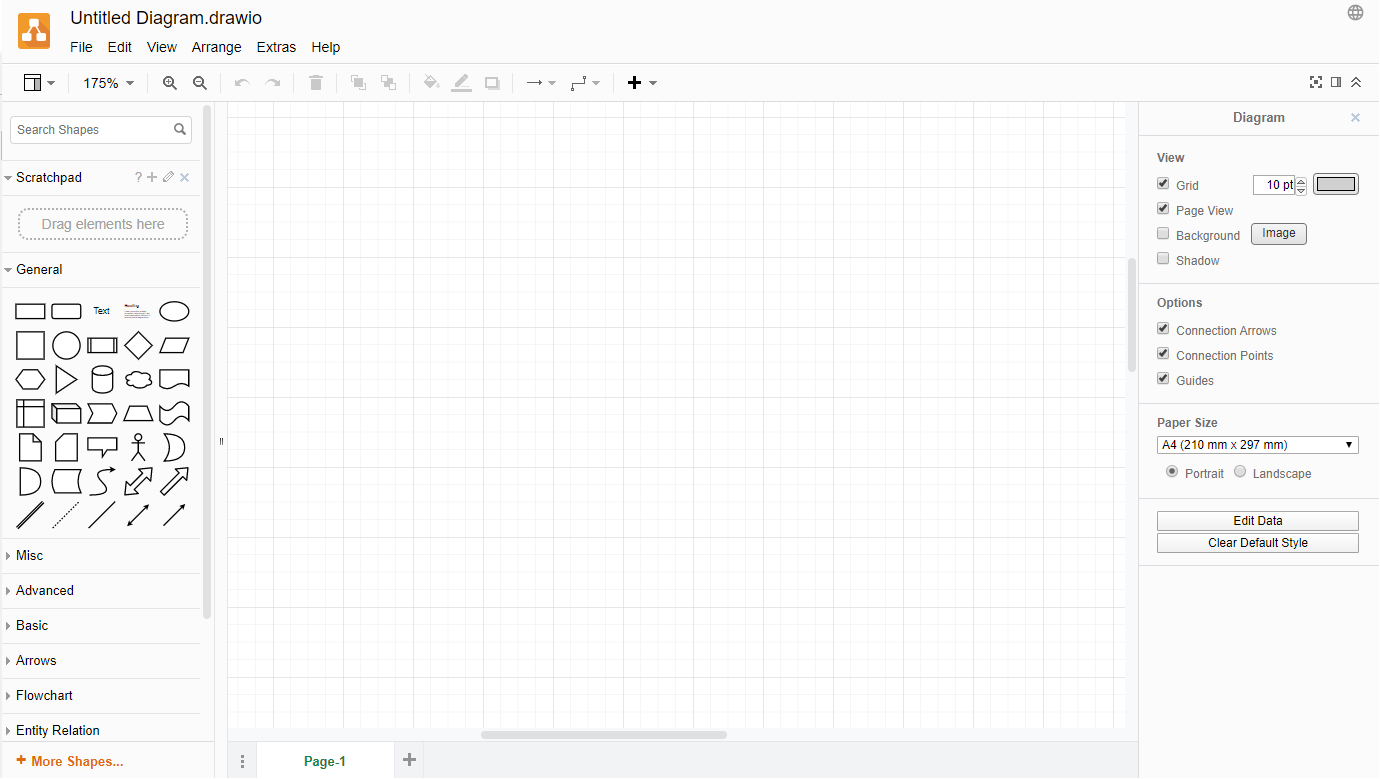
\includegraphics[scale=0.62]{./res/img/draw.png}
		\caption{Schermata principale draw.io}
	\end{figure}

	\subsubsubsection{ESLint}
	ESLint\ped{\textit{G}} è uno strumento di analisi statica per identificare pattern problematici all'interno di codice JavaScript\ped{\textit{G}}. Tale strumento permette inoltre di descrivere e utilizzare regole personalizzate. ESLint\ped{\textit{G}} controlla sia la code quality che eventuali problemi riguardanti lo stile di codifica.
	\begin{center}
		\url{https://eslint.org/}
	\end{center}

	\subsubsubsection{Ethers.js}
	Ethers.js\ped{\textit{G}} è una libreria che consente l'interazione con la blockchain\ped{\textit{G}} Ethereum\ped{\textit{G}} ed il suo ecosistema.
	\begin{center}
		\url{https://docs.ethers.io/ethers.js}
	\end{center}

	\subsubsubsection{Ganache}
	Si tratta di un Ethereum client, con la particolarità di consentire la creazione di una blockchain\ped{\textit{G}} privata finalizzata all'esecuzione di test in locale.
	\begin{center}
		\url{https://www.trufflesuite.com/ganache}
	\end{center}

	\subsubsubsection{Husky}
	Strumento utilizzato per la prevenzione di commit\ped{\textit{G}} dannosi nella Repository\ped{\textit{G}} Git\ped{\textit{G}}.
	\begin{center}
		\url{https://github.com/typicode/husky}
	\end{center}

	\subsubsubsection{Node.js}
	Runtime environment di JavaScript\ped{\textit{G}} open source\ped{\textit{G}}, particolarmente utilizzata all'interno del progetto per l'ascolto di eventi.
	\begin{center}
		\url{https://nodejs.org/it/}
	\end{center}

	\subsubsubsection{NPM}
	Package manager\ped{\textit{G}} utilizzato per l'installazione di strumenti utilizzati durante il progetto.
	\begin{center}
		\url{https://docs.npmjs.com/}
	\end{center}

	\subsubsubsection{Open Zeppelin}
	Libreria composta da smart contract\ped{\textit{G}} ben documentati, utilizzata all'interno del progetto per la scrittura di contratti upgradable.
	\begin{center}
		\url{https://openzeppelin.com/}
	\end{center}

	\subsubsubsection{Ropsten}
	Testnet pubblica usata per test e sperimentazioni su rete Ethereum\ped{\textit{G}}. Permette di essere utilizzata senza preoccuparsi dei costi e senza possedere monete di reale valore.
	\begin{center}
		\url{https://ropsten.etherscan.io/}
	\end{center}

	\subsubsubsection{Serverless}
	Framework\ped{\textit{G}} utilizzato per lo sviluppo, il deploy\ped{\textit{G}} ed il monitoraggio della comunicazione con AWS Lambda\ped{\textit{G}}.
	\begin{center}
		\url{https://www.serverless.com/}
	\end{center}

	\subsubsubsection{Solidity}
	Linguaggio utilizzato per lo sviluppo di smart contract\ped{\textit{G}}.
	\begin{center}
		\url{https://solidity.readthedocs.io/en/v0.6.4/}
	\end{center}

	\subsubsubsection{Truffle}
	Framework\ped{\textit{G}} per lo sviluppo, test e gestione di smart contract\ped{\textit{G}}. Permette la scrittura di test automatici sia in JavaScript\ped{\textit{G}} che in Solidity\ped{\textit{G}}.
	\begin{center}
		\url{https://www.trufflesuite.com/truffle}
	\end{center}

	\subsubsubsection{Visual Studio Code}
	Visual Studio Code è l'IDE\ped{\textit{G}} scelto per la parte di codifica, in particolare tale scelta è dovuta a:
	\begin{itemize}
		\item completa compatibilità con Windows, Linux e macOs: in questo modo tutti i membri del gruppo possono riferirsi ad un unico strumento senza essere vincolati dal sistema operativo da loro utilizzato;
		\item supporto per sistemi di debugging;
		\item integrazione del sistema di versionamento Git\ped{\textit{G}};
		\item numerose estensioni facilmente installabili in grado di coprire la maggior parte delle necessita del gruppo, in particolare per quanto riguarda il calcolo delle metriche:
		\begin{itemize}
			\item \textbf{CodeMetrics}, per il calcolo della complessità ciclomatica in codice Javascript\ped{\textit{G}} e Typescript\ped{\textit{G}}.
			\item \textbf{Solidity Metrics}, per il calcolo della complessità ciclomatica in codice Solidity\ped{\textit{G}}.
			\item \textbf{Comment Counter}, per il rapporto tra linee codice e linee commento.
		\end{itemize}
	\end{itemize}
	\begin{center}
		\url{https://code.visualstudio.com/}
	\end{center}
